\documentclass{article}
\usepackage[utf8]{inputenc}
\usepackage[margin=0.8in]{geometry}

\title{Simple Range Queries}
\author{Justin Zhang}
\date{6 October 2017}

\usepackage{graphicx}

\usepackage{algorithm}
\usepackage{algorithmicx}
\usepackage[noend]{algpseudocode}

\usepackage{tikz}
\usetikzlibrary{calc,shapes.multipart,chains,arrows,positioning}

\tikzstyle{vertex}=[draw,fill=myseagreen,circle,minimum size=24pt,inner sep=0pt]

\tikzstyle{splitvertex}=[draw,fill=myseagreen,circle split,minimum size=24pt]


% for black and white printing; see below
%\definecolor{myseagreen}{RGB}{88,197,191}
%\definecolor{mysalmon}{RGB}{255,160,122}
%\definecolor{myred}{RGB}{255,102,102}
%\definecolor{mypurple}{RGB}{225,145,255}

\definecolor{myseagreen}{RGB}{238,238,238}
\definecolor{mysalmon}{RGB}{204,204,204}
\definecolor{mypurple}{RGB}{170,170,170}

\definecolor{myblack}{RGB}{0,0,0}
\definecolor{mywhite}{RGB}{255,255,255}


\begin{document}

\maketitle

\section{Range Sums}
\subsection{The Problem}
Given a dynamic array, find the sum of a given contiguous range.
Specifically,
\begin{itemize}
    \item \textit{sum}(p,q): Sums indices $p, p+1, ... q-1, q$
    \item \textit{update}(i,v): Updates value at index $i$ to value $v$ 
\end{itemize}

\begin{figure}[h]
\centering
{
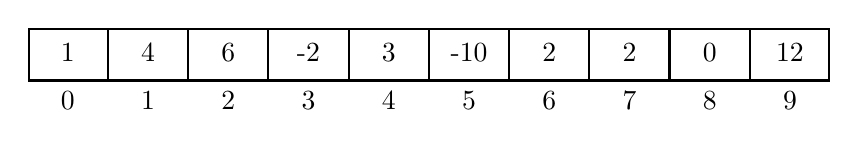
\begin{tikzpicture}[
  thick,
  myrect/.style={
    draw,
    rectangle split,
    rectangle split horizontal,
    rectangle split parts=#1,
    rectangle split part align=left,
    text width=5ex,
    text centered
    },
  mycallout/.style={
    shape=rectangle callout,
    rounded corners,
    fill=mysalmon,
    callout absolute pointer={#1},
    callout pointer width=1cm
  }  
]

\node[myrect=10, rectangle split part fill={mywhite, mywhite, mywhite, mywhite, mywhite, mywhite, mywhite, mywhite, mywhite, mywhite}]
  (array1)
  {
  					\strut 1
  \nodepart{two}	\strut 4
  \nodepart{three}	\strut 6
  \nodepart{four}	\strut -2
  \nodepart{five}	\strut 3
  \nodepart{six}	\strut -10
  \nodepart{seven}	\strut 2
  \nodepart{eight}	\strut 2
  \nodepart{nine}	\strut 0
  \nodepart{ten}	\strut 12
  };
\foreach \Valor [count=\Valori from 0] in {one ,two ,three ,four ,five ,six ,seven ,eight ,nine ,ten }
  \node[below] at (array1.\Valor south) {\Valori};

\end{tikzpicture}
}
\caption{A sample array.}
\end{figure}
For the above array, we might be asked:
\begin{itemize}
    \item \textit{sum}(0, 2): 11
    \item \textit{sum}(5, 8): -6
    \item \textit{update}(8, 6)
    \item \textit{sum}(3, 8): 1
\end{itemize}

\subsection{An $O(n)$ sum, $O(1)$ update solution}
This is the straightforward, naive implementation. Store the values in an array. Given a query:
\begin{itemize}
    \item On \textit{query}(p,q): loop from $p$ to $q$, summing all values in between.
    \item On \textit{update}(i,v): update the array.
\end{itemize}

\subsection{An $O(1)$ sum, $O(n)$ update solution}
Store the values in an array $a$. Create an auxiliary array $b$ such that index $i$ equals \textit{sum}(0, i) -- do this by looping through $a$, keeping a running sum ($b$ stores the \textit{prefix sums} of $a$).
\begin{figure}[h]
\centering
{
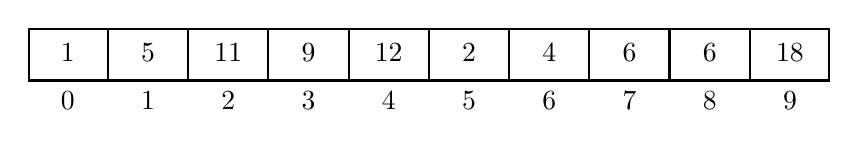
\begin{tikzpicture}[
  thick,
  myrect/.style={
    draw,
    rectangle split,
    rectangle split horizontal,
    rectangle split parts=#1,
    rectangle split part align=left,
    text width=5ex,
    text centered
    },
  mycallout/.style={
    shape=rectangle callout,
    rounded corners,
    fill=mysalmon,
    callout absolute pointer={#1},
    callout pointer width=1cm
  }  
]

\node[myrect=10, rectangle split part fill={mywhite, mywhite, mywhite, mywhite, mywhite, mywhite, mywhite, mywhite, mywhite, mywhite}]
  (array1)
  {
  					\strut 1
  \nodepart{two}	\strut 5
  \nodepart{three}	\strut 11
  \nodepart{four}	\strut 9
  \nodepart{five}	\strut 12
  \nodepart{six}	\strut 2
  \nodepart{seven}	\strut 4
  \nodepart{eight}	\strut 6
  \nodepart{nine}	\strut 6
  \nodepart{ten}	\strut 18
  };
\foreach \Valor [count=\Valori from 0] in {one ,two ,three ,four ,five ,six ,seven ,eight ,nine ,ten }
  \node[below] at (array1.\Valor south) {\Valori};

\end{tikzpicture}
}
\caption{The prefix sums of the array denoted in Figure 1.}
\end{figure}
Given a query:
\begin{itemize}
    \item On \textit{query}(p,q): return $b[q] - b[p-1]$ if $p > 0$, else $b[q]$.
    \item On \textit{update}(i,v): set $a[i]$ to $v$, and recalculate the prefix sums.
\end{itemize}
What if we need range updates? Namely, $update$($i_1$,$i_2$,v) \textit{sums} all elements between indices $i_1$ and $i_2$. 

\subsection{Range updates}

The following is a $O(n)$ sum, $O(1)$ update approach.
Let's assume we start with an array $a$ of all zeros (if we want to start with certain values, we can do $n$ $O(1)$ range updates). Given a query:
\begin{itemize}
    \item On \textit{update}($i_1$,$i_2$,v): Add $v$ to $a[i_1]$. If $i_2 < |a|-1$, subtract $v$ from $a[i_2+1]$.
    \item On \textit{query}(p,q): Notice that setting $a$ to its array of prefix sums $b$ renders the actual values after the update operations. Then, we can loop through $b$ to get the final sum.
\end{itemize}

To make this $O(1)$ sum, $O(n)$ range update, we can calculate the prefix sums of $a$ ($b$) and then the prefix sums of $b$ ($c$) on \textit{update}. This simply does the $O(n)$ computation earlier.

How might we extend prefix sums to two dimensions?

\section{Range Min/Max}
Unlike for range sums, there is no ``prefix min/max" (why?). Thus, the single-update range min/max task can be naively solved only in $O(n)$ range min/max and $O(1)$ update or $O(1)$ range min/max and $O(n^2)$ update. Dynamic programming (sparse tables) can bring this down to $O(1)$ range min/max and $O(n \log n)$ update. Square-root decomposition allows for $O(\sqrt{n})$ range min/max and $O(n)$ update. We won't cover these here, however, because these solutions are more involved.

It's worth noting that there is a $O(n)$ solution to computing all range min/maxes of an arbitrary length $k$ in an array $a$. That is, it computes the minimum of $a[0]...a[k-1], a[1]...a[k], a[2]...a[k+1]$ and so on in $O(n)$. This is the \textit{sliding window maximum} problem, whose solution only requires a deque (double-ended queue).

Let's call the deque $d$. The solution for the maximum variant is as follows:
Loop through the length of $a$ with variable $i$. While $a[i]$ is greater than the back of $d$, pop the back of $d$. Then, push $i$ into the back of $d$. Additionally, while the indices of the front of $d$ are less than or equal to $i-k$, pop from the front of $d$. After these operations, the front of $d$ will be the answer for $a[i-k+1]$ to $a[i]$.

This works because, at any given moment, $d$ contains indices in sorted ascending order with the values of these indices in sorted descending order. For a given index $i$, we remove the newly ineligible values from the front and add the new index from the back. When we add this new index from the back, we remove all indices with values less than $a[i]$ because we know that these indices cannot affect later maximums (concretely, if we have an index $j$ such that $j < i$ and $a[j] < a[i]$, $a[j]$ cannot be the maximum for future ranges because $i$ is closer and $a[i]$ is larger). Thus, the front is the greatest eligible value.

Note that segment trees (with lazy propagation for range updates) can solve all of the above problems (range min/max and sum) in $O(\log n)$ update and $O(\log n)$ query, though its implementation is more involved. We'll cover these later in the year.

\section{Sample problems}
\begin{itemize}
    \item USACO 2014 US Open, Silver, Problem 1: you're given $n$ cows ($2 \leq n \leq 10^5$) positioned along the number line, each either spotted or white. Farmer John can paint spots on any of his white cows. Find the largest contiguous range of cows such that there can be an equal number of white and spotted cows (after painting the spots).
    \item Given an array with length $n$ ($1 \leq n \leq 10^6$), find the largest contiguous range with sum $s$.
    \item USACO 2012 US Open, Silver, Problem 2: Farmer John has been having trouble making his plants grow, and needs your
help to water them properly.  You are given the locations of N raindrops  
($1 \leq N \leq 10^5$) in the 2D plane, where y represents vertical height of
the drop, and x represents its location over a 1D number line:  



Each drop falls downward (towards the x axis) at a rate of 1 unit per
second.  You would like to place Farmer John's flowerpot of width W
somewhere along the x axis so that the difference in time between the
first raindrop to hit the flowerpot and the last raindrop to hit the
flowerpot is at least some amount D (so that the flowers in the pot receive
plenty of water).  A drop of water that lands just on the edge of the
flowerpot counts as hitting the flowerpot.

Given the value of D and the locations of the N raindrops, please compute
the minimum possible value of W.
\end{itemize} 

\end{document}
